\chapter{Metodologia - Métodos de metamodelagem} \label{chap_principios}

A Eq. (\ref{eq:1a}) mostra a relação matemática estabelecida entre uma variável de interesse (ou entrada) $x$ com a variável de saída (ou resposta) $y$ através de uma determinada função (ou modelo) $f$.
\begin{equation}
y = f(x)
\label{eq:1a}
\end{equation}

Para obtermos um metamodelo de $f$, tem-se que obter uma nova função $g$ que irá aproximar o modelo original. Essa relação pode ser expressa da seguinte forma:
\begin{equation}
\hat{y}= {g(x)} \hspace{0.1 cm} \longrightarrow \hspace{0.1 cm} y=\hat{y}+\epsilon
\end{equation}

\noindent onde $\epsilon$ representa o erro de aproximação e $\hat{y}$ é a variável de saída (resposta determinada por um dado metamodelo) que busca a melhor representação do modelo original. 

A metamodelagem deve seguir alguns procedimentos. Segundo \citeonline{Simpson2001}, tais procedimentos perpassam a amostragem, que tem por objetivo a seleção de dados de entrada e saída associados ao modelo original para, posteriormente, determinar qual a função ou o conjunto de funções que irá representar este modelo. Ademais, deve-se realizar o ajuste da função ou funções ao conjunto de dados amostrados. Por fim, é essencial a validação definindo amostras não consideradas na amostragem inicial, nas quais os resultados obtidos através do modelo original e do metamodelo são comparados.

Como mencionado, uma das etapas mais importantes da metamodelagem é a amostragem dos dados de entrada e saída. Assim, deve-se procurar métodos que levam ao menor número possível de amostras para representar o espaço de projeto considerado. Desta forma, um menor gasto computacional é obtido com boa precisão das respostas. 

Na literatura, encontram-se como métodos de amostragem o {\it grid} regular, o Método de Monte Carlo (\textit{Monte Carlo Simulation} - MCS) e o Método do Hipercubo Latino (\textit{Latin Hypercube Sampling} - LHS), que vem a ser uma versão mais simples do MCS, dentre outros. Já quando é necessário definir quais os fatores que mais influenciam a resposta do modelo, o planejamento fatorial é uma boa opção. \textcolor{red}{Ressalta-se que a aplicação dos referidos métodos de amostragem se torna necessária quando não se possuem os dados de entrada e saída do problema considerado. Nesta situação, os dados devem ser selecionados de acordo com o modelo original.}

Neste trabalho, o LHS e o {\it grid} regular foram utilizados e serão abordados a seguir. Posteriormente, as formulações dos métodos de metamodelagem RBF, ANNs, Memória Temporal Hierárquica (\textit{Hierarchical Temporal Memory} - HTM) e \textit{Kriging} são apresentadas.  

\section{Técnicas de amostragem}\label{Amostragem_D}

Dentre as diversas técnicas de amostragem, cita-se a crescente utilização do LHS por ser uma versão mais simples do MCS. O MCS teve o seu desenvolvimento durante a Segunda Guerra Mundial para uso na resolução de problemas vinculados à difusão de nêutrons no projeto da bomba atômica \cite{borges2008}. 

O MCS utiliza uma seleção aleatória de números para que a amostragem seja feita a partir de uma distribuição de probabilidade definida previamente. Por se tratar de um método de seleção aleatória, ele possui chance de amostragem em qualquer ponto da distribuição. Porém, o MCS segue a probabilidade da distribuição selecionada, havendo assim mais amostras no ambiente de maior probabilidade e, consequentemente, poucas amostras na região de menor probabilidade \cite{costa2016}.

Portanto, o MCS consiste na geração de amostras a partir de uma distribuição de probabilidade adotada, seguida pela realização dos cálculos determinísticos utilizando cada amostra gerada, finalizando com resultados e sua análise \cite{lima2011}. Uma vez que este método é conhecido pelo seu alto custo computacional, decorrente da necessidade de uma grande quantidade de iterações para que haja uma boa representação da resposta, surgiu, como alternativa, o LHS.

O LHS tem a finalidade de redução da quantidade de simulações necessárias para obtenção de bons resultados quando comparado ao MCS. Os pontos são gerados de maneira aleatória, garantindo que todas as partes do espaço de projeto \textcolor{red}{sejam representadas}. O intervalo de cada variável de entrada é divido em estratos, sendo as amostras produzidas aleatoriamente proporcionais à probabilidade de cada estrato \cite{queiroz2017}.

No caso do LHS, a quantidade de estratificações é igualada com a quantidade de iterações, não havendo assim substituições. Através da cobertura homogênea do espaço de pontos amostrados, o método fornece convergência mais rápida. Assim, esse método fornece maior precisão e rapidez, quando comparado ao MCS \cite{Pilger2005}.
 
Dessa forma, o LHS possui claras vantagens em melhor amostrar, necessitando de menos iterações e, assim sendo, demandando menor custo computacional. Além disso, outra vantagem reside em sua seleção de valores aleatórios proporcionais aos estratos, tornando as amostras geradas altamente representativas. No entanto, destaca-se que por ser um método aleatório em cada execução as distribuições dos pontos no espaço de projeto modificam-se. 

No presente relatório parcial, o pacote Python {\it Surrogate Modeling Toolbox} (SMT) foi utilizado para a geração das amostras através do LHS. Alguns critérios de amostragem estão disponíveis como, por exemplo, o {\it center} que centraliza os pontos dentro dos intervalos de amostragem; o {\it maximim}, que considera a distância mínima entre os pontos, alocando-os aleatoriamente dentro do seu intervalo; o {\it centermaximin} que considera a distância mínima entre os pontos, porém esses são centralizados dentro dos intervalos\textcolor{red}{,} entre outros \cite{BOUHLEL2019}. 

Outro método de amostragem cuja implementação é considerada mais simples é chamado de {\it grid} regular. Esse método procura preencher o espaço de projeto de forma uniforme, sendo os valores de cada variável de projeto combinados de forma que se associem com os demais valores das outras variáveis \cite{SICCHIERI2019}.

\textcolor{red}{A Fig. \ref{fig:LHS}} apresenta uma comparação de uma amostragem produzida pelo método LHS utilizando as opções {\it center}, {\it maximim} e {\it centermaximin}, bem como pelo método {\it grid} regular. Neste caso, foram consideradas duas variáveis de projeto com o objetivo de mostrar como cada método distribui os pontos de amostragem no espaço definido.
\begin{figure}[H]
\centering
\subfigure[][]{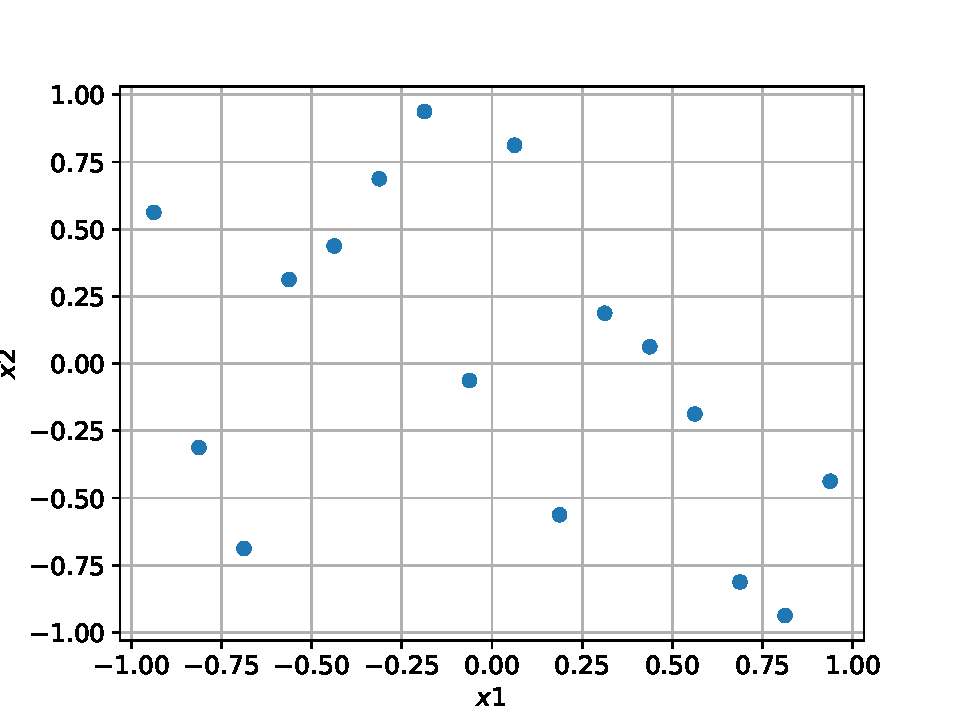
\includegraphics[width=0.4\linewidth]{tatiane/fig_tati/amostragem/fig1.pdf}\label{a}} 
\subfigure[][]{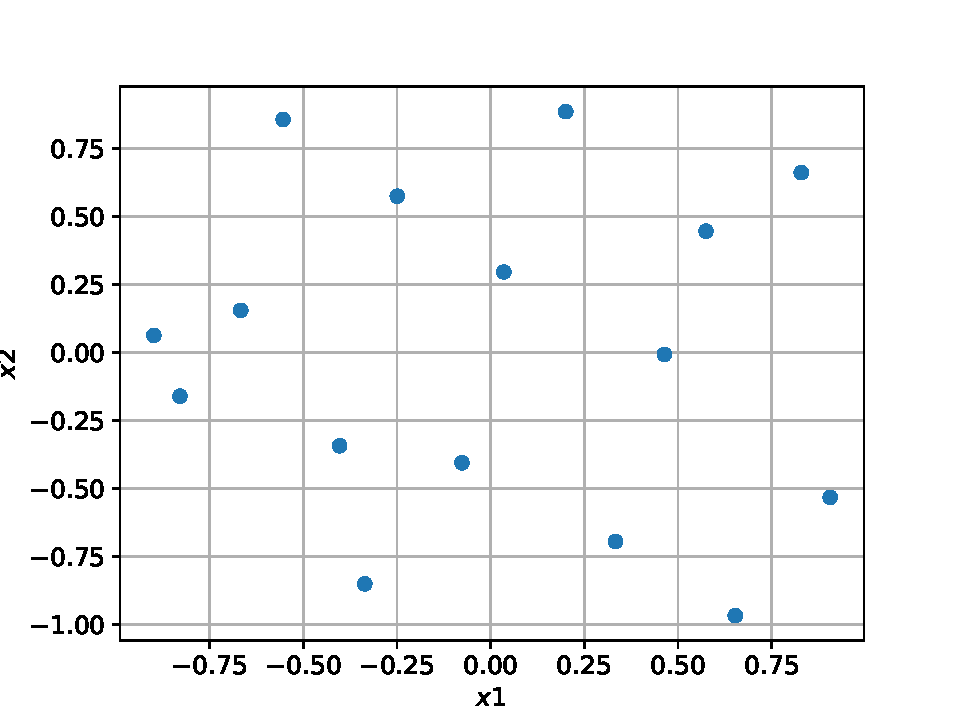
\includegraphics[width=0.4\linewidth]{tatiane/fig_tati/amostragem/fig2.pdf}\label{b}} 
\subfigure[][]{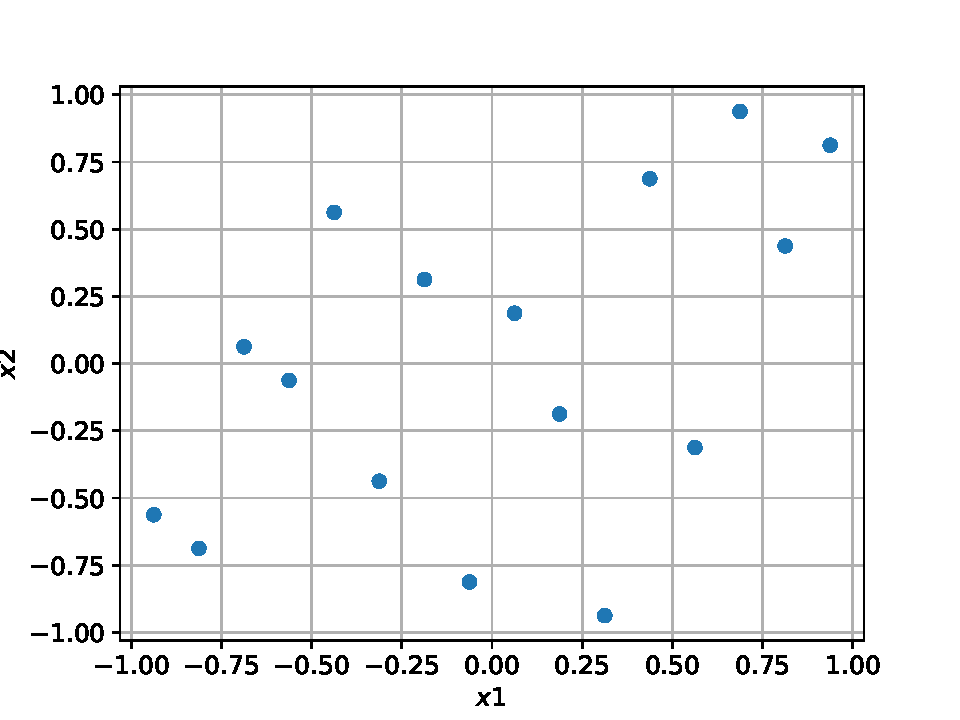
\includegraphics[width=0.4\linewidth]{tatiane/fig_tati/amostragem/fig3.pdf}\label{c}} 
\subfigure[][]{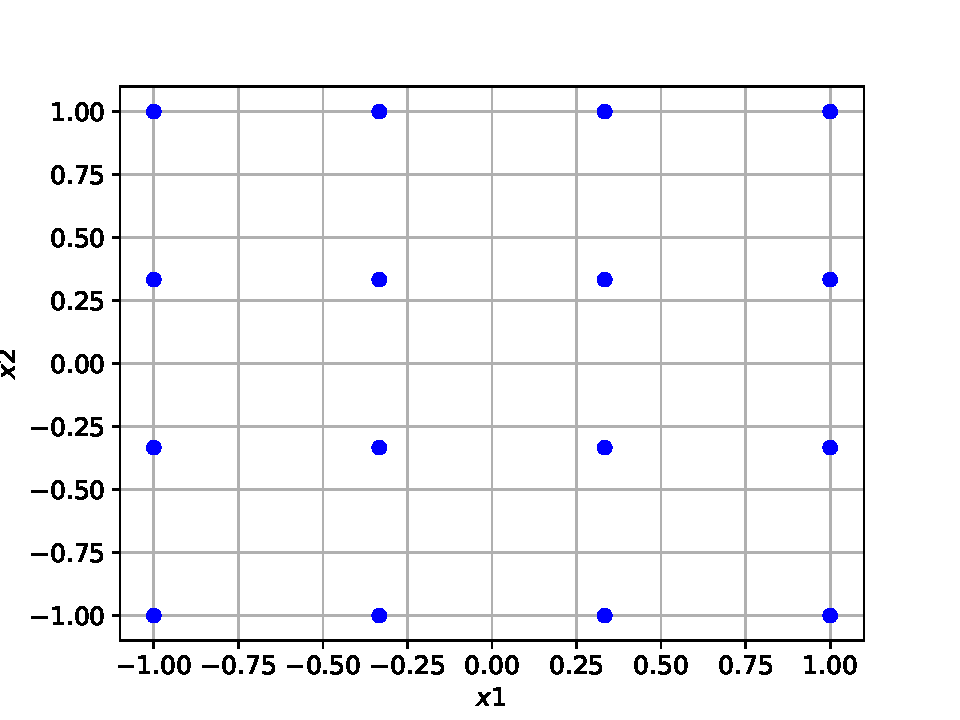
\includegraphics[width=0.4\linewidth]{tatiane/fig_tati/amostragem/fig4.pdf}\label{d}}
\caption{Planejamento amostral pelos métodos a) LHS - center, b) LHS - maximim, c) LHS - centermaximim e d) \textit{grid} regular.}
\label{fig:LHS}
\end{figure}

\section{Técnicas de metamodelagem}\label{metamodelagem_D}

Para construir um metamodelo, deve-se escolher \textcolor{red}{quais  métodos de metamodelagem melhor se encaixam} no problema considerado. \textcolor{red}{Para este fim, existem várias opções como, por exemplo, variantes do método {\it Kriging}, Redes Neurais Artificias, Funções de Base Radial, Rede Neural com a Função de Base Radial, dentre outras}. 

Assim, no trabalho de \citeonline{viana2009} comenta-se que vários artigos compararam o desempenho de vários metamodelos, ressaltando que na maioria das vezes a escolha de qual usar era realizada por experiência, porém uma alternativa satisfatória verificada pelos autores é ajustar vários metamodelos. 

Desta forma, alguns métodos de metamodelagem que vêm sendo aplicados em problemas de engenharia serão abordados mais detalhadamente.

Os metamodelos que serão apresentados a seguir também foram obtidos a partir do pacote SMT. 

\subsection{Metodologia da superfície de resposta - RSM}

A RSM, também denominada de regressão polinomial, utiliza polinômios para a aproximação do modelo original. Ressalta-se que é um dos metamodelos mais simples de ser aplicado e possui baixo custo computacional. Porém, tem a inconveniência de não ser apropriado para modelar comportamentos não lineares. As funções mais utilizadas no RMS são os polinômios de baixa ordem. Assim, para um polinômio de primeira ordem:
\begin{equation}
\hat{y} = {\beta_0}+\sum_{n=1}^{k}{\beta_n}{x_n}
\label{eq:2}
\end{equation}

\noindent onde ${x}_n $ $\in$ ${\Re}^n$, $k$ é o número de variáveis de entrada consideradas ($n=1,...,k$), $\hat{y}$ $\in$ ${\Re}$ e $\beta$ são parâmetros de ajustes ou pesos que ponderam a influência de cada variável de entrada no metamodelo. Para um polinômio de segunda ordem, tem-se:
\begin{equation}
\hat{y} = \beta_0+\sum_{n=1}^{k}{\beta_n}{x_n}+\sum_{n=1}^{k}{{\beta_{nn}}}{x_n^2}+\sum_{n=1}^{k}\sum_{m>n}^{k}{{\beta_{nm}}{x_n}{x_m}}
\label{eq:3}
\end{equation}

\noindent onde $m=n,...,k$.

Para \textcolor{red}{a determinação dos coeficientes dos polinômios apresentados nas Eqs. (\ref{eq:2}) e (\ref{eq:3})}, utiliza-se o método dos mínimos quadrados. Este método minimiza a soma de desvio quadrático dos valores previstos em relação aos valores reais por meio da seguinte relação:
\begin{equation}
\beta= [{X^T}X]^{-1}{X}^Tz
\label{eq:4}
\end{equation}

\noindent $X$ representa a matriz de entrada de dados e $z$ é um vetor coluna que contém a medida de desempenho em cada ponto \cite{myers2016}. \citeonline{KLEIJNEN2015} ressalta que o estimador de mínimos quadrados existirá somente se $ {[{X^T}X]}^{-1}$ existir. 

\subsection{Função de base radial - RBF}

A técnica de metamodelagem RBF é baseada em interpolação. Este método utiliza uma combinação linear de funções de base, as quais dependem da distância euclidiana entre o ponto de previsão e o de treinamento \cite{BOUHLEL2019,sun2017,PINA2010}. Um metamodelo obtido através do RBF é dado por: 
\begin{equation}
\hat{y}=\sum_{n=1}^{k}{\beta_n}f_r{||x-{x_n}||}
\label{eq:5}
\end{equation}

\noindent onde ${\beta_n}$ representa os coeficientes desconhecidos associados \textcolor{red}{às} funções de base radial $f_r$ que servem como fatores de ponderação ou peso; $ ||x -{x}_n||$ é a norma euclidiana entre o ponto que se deseja prever $x$ e o chamado centro da base ${x}_n$. Normalmente, ${x}_n$ é definido como sendo o centro das amostras usadas para o treinamento do metamodelo.

A Eq. (\ref{eq:5}) pode ser acrescentada de funções polinomiais com o objetivo de capturar as tendências dos dados. Assim, 
\begin{equation}
\hat{y}=\sum_{n=1}^{k}{\beta_n}f_r{||x-{x_n}||}+\sum_{q=1}^{s}{\alpha_q}p_q(x)
\label{eq:6}
\end{equation}

\noindent sendo que ${p}_q$ representa o vetor de coeficientes do polinômio, ${\alpha}_q$ representa o vetor de pesos da função polinomial e $s$ é o número de termos polinomiais ($q=1,...,s$). Utilizando-se o RBF dado pela Eq. (\ref{eq:6}), tem-se uma combinação linear de funções de base radial $f_r$ e termos polinomiais ${p}_q$ com coeficientes ponderados ${\alpha}_q$.

A Tab. \ref{funcbase} apresenta as principais funções de base radial encontradas na literatura \cite{BOUHLEL2019}. \\

\begin{table}[H]
	\caption{Principais funções de base radial.} \label{funcbase} 
	\centering
	\begin{tabular}{ c c c c}
		\hline
		Funções de base & Formulação \\
		\hline \\[2pt] 
		Gaussiana & $ \exp\left(\frac{-{{d}^2}} {2{\theta}^2}\right)  $ \\[7pt]
		Cúbica &  ${d^3}$ \\[7pt] 
		Multiquadrática Inversa &  $\frac{1} {\sqrt{d^{2}+\theta^{2}}}$ \\[7pt]
		Multiquadrática &  ${\sqrt{d^{2}+\theta^{2}}}$ \\[7pt]
		\hline
	\end{tabular}
\end{table}

\noindent onde $d=||x-x_{i} ||$ e $\theta$ representa um parâmetro que controla a largura das funções de base radial. A função a ser escolhida depende da natureza dos dados e da precisão de ajuste esperada. É importante ressaltar que processos de minimização podem ser empregados para determinar o valor de $\theta$, bem como os valores de ${\beta_n}$ e ${\alpha}_q$. 

De acordo com \citeonline{ma2008}, o RBF tem como vantagem um bom desempenho em precisão, robustez e menor tamanho da amostra quando comparado aos métodos RSM e {\it Kriging}. Como desvantagem, os autores ressaltaram o gasto computacional. 

\subsection{Redes neurais artificiais - ANNs}

As ANNs vêm sendo utilizadas como outra classe de técnicas de metamodelagem para a aproximação de funções complexas.  De acordo com \citeonline{sampaio2009}, ANNS são algoritmos baseados no mecanismo do cérebro, ou ainda, são inspiradas em redes neurais biológicas cerebrais, sendo capazes de executar as mais diversas tarefas como, por exemplo, aproximar funções, reconhecer padrões, entre outras. \citeonline{Simpson2001} mostra que as ANNs mais comuns são as de múltiplas camadas (\textit{multilayer perceptron}), por serem aplicadas na resolução de problemas não lineares. 

De acordo com \citeonline{braga2007}, uma rede neural é constituída por neurônios artificiais que possuem uma função de ativação gerando uma resposta. Os neurônios são dispostos em camadas e são ligados entre si. Estas conexões estão associadas \textcolor{red}{a} coeficientes chamados de pesos, em que o ajuste dos pesos é realizado por treinamento. 

A Fig. \ref{fig:rd} mostra a representação de um neurônio. As entradas são denotadas por ${x}_1$, ${x}_2$, $...$, ${x}_n$; e a variável de saída é $\hat{y}$. Neste caso, o vetor de entrada é multiplicado pelos pesos ${w}_1$, ${w}_2$, $...$, ${w}_n$; $\beta$ é um peso independente \cite{sampaio2009,PINA2010}. \\

\begin{figure}[!htbp]
	\centering
	{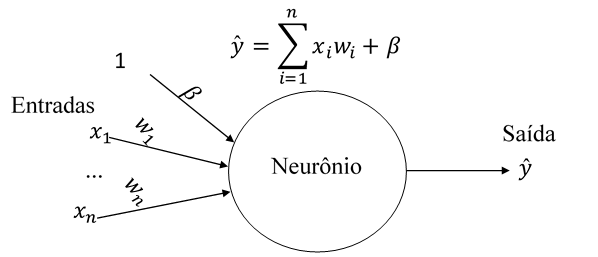
\includegraphics[width=0.5\linewidth]{tatiane/fig_tati/redeneural/neuronio.png}}\caption{Representação de um neurônio. Adaptada de \citeonline{sampaio2009}.} 
	\label{fig:rd}
\end{figure}

Diversas são as funções que podem ser utilizadas como ativadoras de um neurônio, como por exemplo, função linear, função lógica e sigmóide. A função ativadora tem como finalidade ser um limitante aplicado na amplitude de saída do neurônio.

Segundo \citeonline{PINA2010}, a sigmóide é a função mais utilizada, sendo que uma função para ser deste tipo não pode exceder limites inferiores e superiores, além de ser monótona crescente. Desta forma, quando o valor de entrada cresce o valor da função também cresce e vice-versa. São exemplos de funções sigmóides a função logística e a tangente hiperbólica.

A arquitetura das ANNs é definida conforme as conexões entre os neurônios, cuja rede é dividida em camadas de neurônios, podendo ser simples {\it (single layer)} ou multicamadas {\it (multi-layer)}. Segundo \citeonline{PINA2010}, uma rede de camada simples possui apenas uma camada de conexões entre a entrada e a saída, como ilustrado na Fig. \ref{fig:cams}. Diferentemente, uma ANN de multicamadas é composta por várias redes de camadas simples, nas quais os neurônios de camadas adjacentes são conectados (veja a Fig. \ref{fig:multcama}).

\begin{figure}[H]
	\centering
	{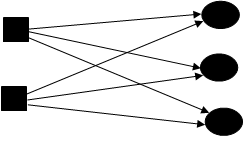
\includegraphics[width=0.3\linewidth]{tatiane/fig_tati/redeneural/camsimp.png}} 
	\caption{Representação de uma ANN de camada simples. Adaptada de 
	\citeonline{PINA2010}.} 
	\label{fig:cams}
\end{figure}

\begin{figure}[H]
	\centering
	{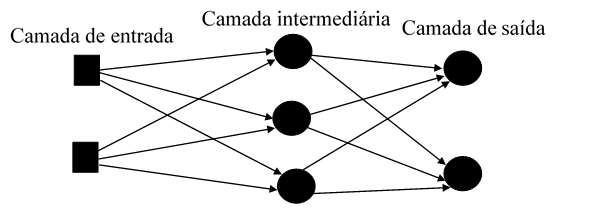
\includegraphics[width=0.6\linewidth]{tatiane/fig_tati/redeneural/multicamadas}}\caption{Representação de uma ANN de multicamadas. Adaptada de \citeonline{PINA2010}.} 
	\label{fig:multcama}
\end{figure}

Segundo \citeonline{VILLAR2016}, uma ANN multicamadas opera da seguinte maneira:

\begin{itemize}
\item As camadas de entrada são responsáveis por receber as informações de uma fonte externa e passar as informações para o processamento;
\item A camada intermediária ou oculta, recebe as informações da camada de entrada e realiza todo o processo de informação, sendo que o tamanho destas camadas e o número de camadas ocultas entre a entrada e saída da ANN é de escolha do projetista; 
\item A camada de saída recebe as informações processadas da rede e apresenta os resultados.

\end{itemize}

Os neurônios podem ser associados, formando diferentes estruturas ou topologias. A mais comumente utilizada é denominada de {\it feedforward}. Nessa estrutura, os neurônios são agrupados em camadas, o sinal percorre a ANN em uma única direção e os neurônios da mesma camada não são conectados \cite{Simpson2001}. De acordo com \citeonline{PINA2010}, em ANNs recorrentes, a saída de um neurônio pode ser utilizada como entrada para neurônios da mesma camada ou para camadas anteriores.

O aprendizado das ANNs é realizado para determinar os melhores valores dos pesos que se adequam ao problema associado. Este processo pode ser supervisionado ou não supervisionado. 

No processo de aprendizado supervisionado, a rede é treinada através do fornecimento dos valores de entrada e de saída desejados em relação aos pesos. Estes são ajustados por meio de um processo de minimização de erro. Sendo assim, compara-se a saída desejada com a saída da rede. No processo de aprendizado não supervisionado, somente os valores de entrada são fornecidos \cite{PINA2010}.

As ANNs podem ser utilizadas como modelos substitutos de problemas computacionais de alto custo computacional. O metamodelos baseados em ANNs tem como desvantagens a dificuldade de selecionar a estrutura mais apropriada, qual a função de ativação a ser utilizada e a quantidade de termos necessários.

\subsection{Redes neurais com função de base radial}

As ANNs com RBF são um caso particular de metamodelos que vêm sendo utilizados. Segundo \citeonline{fonseca2017}, este metamodelo possui três camadas: a camada de entrada, na qual os dados são introduzidos na rede; a intermediária, que realiza a transformação não linear do espaço de entrada para um espaço escondido; e a camada de saída, que produz a resposta da rede neural. A função de ativação de cada neurônio é uma função de base radial, isto é, representa a distância entre o vetor de entrada e o centro do neurônio. Logo, a saída da rede é expressa como \cite{viana2008,fonseca2009}:
\begin{equation}
\hat{y}= \sum_{n=1}^{N}w_n{f}_r{||x-{c_n}||}
\label{eq:10}
\end{equation}

\noindent onde $N$ representa o número de neurônios da camada oculta (intermediária), ${c}_n$ são os centros da função de base radial dos neurônios e ${w}_n$ são os pesos que ponderam cada ativação da camada intermediaria para a camada de saída, ${f}_i$ são as funções de base radial, sendo que algumas foram descritas na Tabela \ref{funcbase}.

\subsection{Redes Neurais de Memória de Longo Prazo - LSTM}

Segundo \citeonline{cetax}, as Redes Neurais de Memória de Longo Prazo (\textit{Long Short-Term Memory} - LSTM) são um tipo especial de ANNs proposto por \citeonline{Hochreiter}. Sua principal característica é a capacidade de recordar informações por longos períodos de tempo. Dentre a vasta gama de aplicações, destacam-se reconhecimento de escrita, tradução, modelagem acústica de voz, predição de estruturas proteicas, análise de vídeos, previsão de enchentes e previsões de comportamento do mercado financeiro, sendo o estado da arte das redes neurais para aprendizado de sequências. Apesar das inúmeras variantes da arquitetura LSTM que foram concebidas desde seu surgimento, \citeonline{Greff} observa que nenhuma representa um ganho significativo em relação à proposta original.

De acordo com \citeonline{Hochreiter}, nos tipos convencionais de redes neurais recorrentes, os sinais de erro que retroalimentam a rede \textcolor{red}{tendem a divergir ou serem dissipados}, dependendo dos valores dos pesos adotados. As redes LSTM são projetadas para serem capazes de superar tais erros de propagação, sendo capazes de aprender a associar informações separadas por até 1000 passos de tempo, ainda que na presença de ruído. Mesmo nessas condições, não há perda da memória de curto prazo. Tais qualidades são possíveis graças ao uso de um eficiente algoritmo baseado em gradientes e uma arquitetura que garante um fluxo de erro constante através dos estados internos de unidades especiais, as quais serão discutidas adiante.

Assim como nas ANNs, a arquitetura das LSTMs são compostas por uma estrutura em cadeia que repete os mesmos módulos. No entanto, para assegurar o fluxo constante do erro, em uma LSTM cada módulo é composto por três portões (\textit{gates}): portão de entrada (\textit{input gate}), portão de saída (\textit{output gate}) e portão de esquecimento (\textit{forget gate}).  Além dos portões, um bloco de rede LSTM também incorpora uma célula CEC (\textit{Constant Error Carousel}), uma função de ativação de saída (\textit{output activation function}), uma entrada de informações para o bloco (\textit{block input}) e conexões do tipo \textit{peephole}. A saída do bloco (\textit{block output}) normalmente é conectada à entrada e aos demais blocos. A Fig. 3.5 esquematiza tais unidades.

\begin{figure}[H]
	{\centering}
	{\includegraphics[width=1\linewidth]{figuras_LSTM/Greff_Fig_1}}
	{\caption{Esquema detalhado de uma unidade de ANN recorrentes simples (SRN) e um bloco de LSTM. Fonte: \citeonline{Greff}.}}
	{\label{fig:lstmcell}}
\end{figure}

Segundo \citeonline{Hochreiter}, os portões de entrada controlam o fluxo de sinais de erro que entram em uma célula de memória a fim de evitar conflito de pesos. Os portões de saída por sua vez, controlam como os sinais de erro deixam essa célula. Em outras palavras, a rede usa os portões de entrada para decidir quando manter ou sobrescrever informações na célula, e os portões de saída para decidir quando permitir o acesso à informação ou prevenir outras unidades de serem perturbadas por essa célula.

Sinais de erro aprisionados em uma célula CEC não podem ser alterados, mas diferentes sinais de erro passando pela célula, em diferentes tempos, podem ser sobrepostos por meio dos portões de saída. Os portões de saída têm que aprender quais erros armazenar em suas células. Da mesma forma, os portões de entrada devem aprender quando permitir a entrada de sinais de erro. Os portões de esquecimento possibilitam às células retornarem aos seus valores originais, permitindo o aprendizado de tarefas \textcolor{red}{contínuas}. 

Em seu trabalho, \citeonline{Greff} concluem que a formulação dos portões é o parâmetro de maior influência no desempenho da LSTM. Os autores definem os pesos de cada unidade em alimentação direta na forma:
\begin{itemize}
	\item Pesos das entradas: $\mathbf{W_z, W_i, W_f, W_o}\in \mathbb{R}^{N \times M}$;
	\item Pesos das conexões recorrentes: $\mathbf{R_z, R_i, R_f, R_o}\in \mathbb{R}^{N \times N}$;
	\item Pesos das conexões \textit{peepholes}: $\mathbf{p_i, p_f, p_o}\in \mathbb{R}^{N}$;
	\item Pesos das influências (\textit{bias}): $\mathbf{b_z, b_i, b_f, b_o}\in \mathbb{R}^{N}$;
\end{itemize}
onde $x^t$ é o vetor de entradas no tempo $t$, $N$ o número de blocos LSTM e $M$ o número de entradas.

As equações dos vetores na alimentação direta, segundo \citeonline{Greff}, são escritas como:
\begin{equation}
\begin{array}{lr}
%\hline
\mathrm{\overline{\mathbf{z}}^t = \mathbf{W_z} \mathbf{x}^t + \mathbf{R_z} \mathbf{y}^{t-1}+\mathbf{b_z} 				    							}& 						\\
\mathrm{z^t = g(\overline{\mathbf{z}}^t)																												}& \textit{Entrada do bloco} \\ %\hline
\mathrm{\overline{\mathbf{i}}^t = \mathbf{W_i} \mathbf{x}^t + \mathbf{R_i} y^{t-1} + \mathbf{p_i} \odot \mathbf{c}^{t-1} + \mathbf{b_i}				}& 						\\
\mathrm{i^t = \sigma(\overline{\mathbf{i}}^t) 																											}& \textit{Portão de entrada} 	\\ %\hline
\mathrm{\overline{\mathbf{f}}^t = \mathbf{W_f} \mathbf{x}^t + \mathbf{R_f} \mathbf{y}^{t-1} + \mathbf{p_f} \odot \mathbf{c}^{t-1} + \mathbf{b_f}	}&						\\
\mathrm{f^t = \sigma(\overline{\mathbf{f}}^t) 																											}& \textit{Portão de esquecimento} \\ %\hline
\mathrm{\mathbf{c}^t = \mathbf{z}^t \odot \mathbf{i}^{t} + \mathbf{c}^{t-1} \odot \mathbf{f}^t													}&\textit{Célula}			\\ %\hline
\mathrm{\overline{\mathbf{o}}^t = \mathbf{W_o} \mathbf{x}^t + \mathbf{R_o} \mathbf{y}^{t-1} + \mathbf{p_o} \odot \mathbf{c}^{t} + \mathbf{b_o}  		}&						\\ 
\mathrm{\mathbf{o}^t = \sigma(\overline{\mathbf{o}}^t) 																									}& \textit{Portão de saída} \\	%\hline	
\mathrm{\mathbf{y}^t = h(\mathbf{c}^t)\odot \mathbf{o}^t																							}& \textit{Saída do bloco}\\		%\hline
\end{array}
\end{equation}

Nas relações acima, $\mathrm{\sigma}$ é a função sigmoide ($\sigma(x)=\frac{1}{1+e^{-x}}$). As funções de ativação  $\mathrm{g}$ e $\mathrm{h}$ são do tipo tangente hiperbólica ($\mathrm{g(x)=h(x)=tanh(x)}$). O operador $\odot$ indica o produto de vetores ponto a ponto.

No processo de retroalimentação dos blocos LSTM, os deltas são calculados como:
\begin{equation}
\begin{array}{ll}
\mathrm{\delta \mathbf{y}^t =} & \mathrm{\Delta^t + \mathbf{R_z}^T \delta z^{t+1} + \mathbf{R_i}^T \delta i^{t+1} \mathbf{R_f}^T\delta f^{t+1} + \mathbf{R_o}^T \delta o^{t+1} }\\

\mathrm{\delta \overline{\mathbf{o}}^{t}=}&\mathrm{\delta \mathbf{y}^{t} \odot h\left(\mathbf{c}^{t}\right) \odot \sigma^{\prime}\left(\overline{\mathbf{o}}^{t}\right)}\\

\mathrm{ \delta \mathbf{c}^{t}=}&\mathrm{ \delta \mathbf{y}^{t} \odot \mathbf{o}^{t} \odot h^{\prime}\left(\mathbf{c}^{t}\right)+\mathbf{p}_{o} \odot \delta} \overline{\mathbf{o}}^{t}+\mathbf{p}_{i} \odot \delta \overline{\mathbf{i}}^{t+1} \\ &\mathrm{+\mathbf{p}_{f} \odot \delta \overline{\mathbf{f}}^{t+1}+\delta \mathbf{c}^{t+1} \odot \mathbf{f}^{t+1} }\\

\delta \overline{\mathbf{f}}^{t}=&\mathrm\delta \mathbf{c}^{t} \odot \mathbf{c}^{t-1} \odot \sigma^{\prime}\left(\overline{\mathbf{f}}^{t}\right) \\

\delta \overline{\mathbf{i}}^{t}=&\mathrm\delta \mathbf{c}^{t} \odot \mathbf{z}^{t} \odot \sigma^{\prime}\left(\overline{\mathbf{i}}^{t}\right) \\

\delta \overline{\mathbf{z}}^{t}=&\mathrm\delta \mathbf{c}^{t} \odot \mathbf{i}^{t} \odot g^{\prime}\left(\overline{\mathbf{z}}^{t}\right)

\end{array}
\end{equation}

\noindent onde $\Delta^t$ é o vetor de deltas passado pela camada precedente. 

Finalmente, sendo $\star$ qualquer $\{ \overline{\mathbf{z}}, \overline{\mathbf{i}}, \overline{\mathbf{f}}, \overline{\mathbf{o}} \}$, os gradientes dos pesos são calculados na forma:
\begin{equation}
\begin{array}{llll} 
\delta \mathbf{W}_{\star}= 	&\sum_{t=0}^{T}\left\langle\delta \star^{t}, \mathbf{x}^{t}\right\rangle 		& \delta \mathbf{p}_{i}=& \sum_{t=0}^{T-1} \mathbf{c}^{t} \odot \delta \overline{\mathbf{i}}^{t+1} \\
\delta \mathbf{R}_{\star}=	& \sum_{t=0}^{T-1}\left\langle\delta \star^{t+1}, \mathbf{y}^{t}\right\rangle 	& \delta \mathbf{p}_{f}=& \sum_{t=0}^{T-1} \mathbf{c}^{t} \odot \delta \overline{\mathbf{f}}^{t+1} \\
\delta \mathbf{b}_{\star}=	& \sum_{t=0}^{T} \delta \star^{t} 												& \delta \mathbf{p}_{o}=& \sum_{t=0}^{T} \mathbf{c}^{t} \odot \delta \overline{\mathbf{o}}^{t}
\end{array}
\end{equation}

\citeonline{ElSaid} investiga a aplicação de redes LSTM aplicadas na predição de vibração de turbinas de motores aeronáuticos. O autor propôs três arquiteturas de rede e uma arquitetura que foi otimizada por um algoritmo heurístico de colônia de formigas (ACO). As redes foram treinadas por meio de um grande banco de dados de sinais temporais provenientes de dados gravados em voo (FDR). Dentre os sinais disponíveis, foram utilizados quinze para o treinamento da rede:
\begin{enumerate}
	\setlength{\itemsep}{0pt}
	\setlength{\parskip}{0pt}
	\item Altitude [ALT];
	\item Ângulo de ataque (AOA);
	\item Pressão de sangria (BPRS);
	\item Temperatura de entrada na turbina (TIT);
	\item Número de Mach (M);
	\item Velocidade de rotação do eixo primário (N1);
	\item Velocidade de rotação do eixo secundário (N2);
	\item Pressão do óleo do motor (EOP);
	\item Quantidade de óleo do motor (EOQ);
	\item Temperatura do óleo do motor (EOT);
	\item Rolagem da aeronave (Roll);
	\item Temperatura total do ar (TAT);
	\item Direção do vento (WDir);
	\item Velocidade do vento (WSpd);
	\item Vibração do motor (Vib)
\end{enumerate}

As redes propostas pelos autores foram projetadas para predizer a vibração do motor em $5 \ s$, $10 \ s$ e $20 \ s$ no futuro. Cada um dos 15 parâmetros FDR é representado por um nó na entrada da rede neural. Um nó adicional é utilizado para tendência. Nas três arquiteturas propostas, são utilizadas células LSTM que recebem tanto uma entrada inicial dos dados de voo em algum momento no passado ou a saída de uma célula em uma camada inferior, quanto a saída de células anteriores na mesma camada. A Fig. 3.6 ilustra a arquitetura explicada.

\textcolor{red}{Nas arquiteturas propostas, cada célula tem três portões (portões de entrada, saída e de esquecimento) para controlar o fluxo de informação, e uma célula de memória que possibilita o uso do fluxo de informações do passado nas predições atuais. Os nós são responsáveis pela entrada ou saída de uma informação na célula, no caso, cada nó poderá receber um dos 15 parâmetros FDR escolhidos. Um neurônio é uma função matemática que busca modelar o funcionamento de um neurônio biológico. Tipicamente o neurônio computa a soma ponderada de suas entradas e alimenta uma função de ativação. A célula é o conjunto de entidades que compõem uma unidade LSTM, ou seja, seus nós, portões, célula CEC e demais funções}.

Na primeira arquitetura proposta por \citeonline{ElSaid}, o primeiro nível recebe a entrada de dez séries temporais (o instante atual mais nove anteriores). A saída do primeiro nível alimenta o segundo nível e é considerada a primeira camada oculta. O segundo nível da rede reduz o número de nós, das 16 entradas (15 nós de entrada mais um de \textcolor{red}{tendência}) por célula para apenas um nó por célula. A saída do segundo nível é considerada a segunda camada oculta. 

\begin{figure}[H]
	\centering
	{\includegraphics[width=1\linewidth]{figuras_LSTM/ACO_LSTM_Turbine_Vibration_fig2_edit_a}}
	{\caption{Visão geral da arquitetura de uma rede LSTM. Adaptado de: \citeonline{ElSaid}.}}
	\label{fig:lstm_aco_arq}
\end{figure}

Finalmente a saída do segundo nível apresenta 10 nós (um nó por célula). Estes nós alimentam um nerônio final, no terceiro nível, para computar a saída de toda a rede. 

A segunda arquitetura é semelhante à primeira, mas sem o terceiro nível. Nesse caso, uma média da saída do segundo nível é realizada para computar a saída da rede, como um todo. 

Por fim, a terceira arquitetura apresenta a rede mais profunda. Vinte séries temporais alimentam o primeiro nível. A saída do primeiro nível alimenta as entradas do segundo, que por sua vez, realiza os mesmos procedimentos do primeiro nível, dando chance para decisões mais abstratas. No terceiro nível, o número de entradas é reduzido de 16 para apenas um nó por célula. Finalmente, a saída do terceiro nível apresenta 20 nós, que alimentam um neurônio no quarto nível para computar a saída da rede. As camadas ocultas são as saídas do primeiro, segundo e terceiro níveis. A Fig. \ref{fig:lstm_aco_3arqs} esquematiza as redes propostas.
\begin{figure}[H]
	\centering
	{\includegraphics[clip,trim={0 7cm 0 0},width=0.9\linewidth]{figuras_LSTM/ACO_LSTM_Turbine_Vibration_fig7}}
\end{figure}

\begin{figure}[H]
	\centering
	{\includegraphics[clip,trim={0 0 0 12.3cm},width=0.9\linewidth]{figuras_LSTM/ACO_LSTM_Turbine_Vibration_fig7}}
	\caption{Três arquiteturas propostas. Fonte: \citeonline{ElSaid}.}
	\label{fig:lstm_aco_3arqs}
\end{figure}

%\begin{figure}
%	\centering
%	{\includegraphics[width=0.9\linewidth]{figuras_LSTM/ACO_LSTM_Turbine_Vibration_fig7}}
%	\caption{Três arquiteturas propostas. Fonte: \citeonline{ElSaid}.}
%	\label{fig:lstm_aco_3arqs}
%\end{figure}
\citeonline{ElSaid} apresenta, por meio da Fig. \ref{fig:lstm_aco_ems}, o resultado do erro médio quadrático (veja a Eq. (\ref{eq:erroMSE})) para as três arquiteturas propostas.

\begin{equation}
 \label{eq:erroMSE}
 \textnormal{EMS} = \frac{0,5 \times \sum\left( \textnormal{Vibração real} - \textnormal{Vibração predita} \right)^2}{\textnormal{Segundos de teste}}
 \end{equation}
 
 Inicialmente, todas as arquiteturas foram treinadas com 575 períodos, entretanto, períodos adicionais foram \textcolor{red}{examinados para a arquiteturas III}. Nos resultados preliminares, o conjunto de dados de vibração foram divididos em 28 voos, com um total de 41431 segundos de dados para treinamento e 38126 segundos de dados para teste.

\begin{figure}[H]
	\centering
	{\includegraphics{figuras_LSTM/ACO_LSTM_Turbine_Vibration_fig14}}
	\caption{Erro médio quadrático durante o processo de treinamento das três arquiteturas para predições de 1, 5, 10 e 20 segundos no futuro. Fonte: \citeonline{ElSaid}.}
	\label{fig:lstm_aco_ems}
\end{figure}

\textcolor{red}{A Fig. \ref{fig:lstm_aco_results1} compara os resultados obtidos pelas três arquiteturas e os valores reais de vibração. Como exemplo, foram selecionados os resultados para quatro voos. A Fig. \ref{fig:lstm_aco_results2} apresenta o mesmo tipo de análise para um único voo}.

\begin{figure}[H]
	\centering
	{\includegraphics{figuras_LSTM/ACO_LSTM_Turbine_Vibration_fig15}}	
	\caption{Resultados das três arquiteturas para 1, 5, 10 e 20 segundos no futuro para uma seleção de voos. Adaptado de: \citeonline{ElSaid}.}
	\label{fig:lstm_aco_results1}
\end{figure}

Segundo \citeonline{ElSaid}, por meio das figuras \ref{fig:lstm_aco_results1} e \ref{fig:lstm_aco_results2} é possível inferir que a arquitetura I se mostra a mais precisa para a predição da vibração. Os autores também observam que a predição de picos maiores é mais precisa que a predição de picos menores, o que sugere que a rede neural apresente a tendência de aprender mais sobre valor crítico máximo de vibração, o que é benéfico para o problema estudado.

A arquitetura II apresentou as predições menos precisas. Apesar de conseguir predizer a maioria das vibrações, o desempenho para a predição de picos (tanto altos quanto baixos) foi fraco. Os autores atribuem essa característica ao uso do operador média na saída da segunda camada.

\begin{figure}[H]
	\centering
	{\includegraphics{figuras_LSTM/ACO_LSTM_Turbine_Vibration_fig16}}
	\caption{Resultados das três arquiteturas para 1, 5, 10 e 20 segundos no futuro para um único voo. Adaptado de: \citeonline{ElSaid}.}
	\label{fig:lstm_aco_results2}
\end{figure}

A arquitetura III, diferentemente das demais, apresenta uma camada adicional e 20 segundos de memória do passado. Embora apresente maior custo computacional e seja mais propícia para aprendizado mais profundo, os resultados não foram tão bons quanto esperado, na visão dos autores. Uma possível explicação, de acordo com  \citeonline{ElSaid}, é que o maior potencial de aprendizado da arquitetura III pode não ter sido aproveitado devido à maior dificuldade de treinamento.

Uma vez que a arquitetura I apresentou os melhores resultados, \citeonline{ElSaid} a escolheu para ser otimizada pelo método ACO. O procedimento utilizado para a otimização foge do escopo do presente relatório, mas pode ser encontrado no texto dos autores. A Fig. \ref{fig:lstm_aco_results3} mostra o resultado obtido pela arquitetura I e pela versão otimizada. 

\begin{figure}[H]
	\centering
	
	{\includegraphics[width=0.5\linewidth]{figuras_LSTM/ACO_LSTM_Turbine_Vibration_fig17}}
	
	\caption{Comparação entre resultados da arquitetura I e da rede otimizada para 10 segundos no futuro. Fonte: \citeonline{ElSaid}.}
	\label{fig:lstm_aco_results3}
\end{figure}

\textcolor{red}{Os autores obtiveram uma melhoria de $1,34\%$ no erro para a predições de 10 segundos, o que é observado pelo melhor ajuste apresentado na Fig. \ref{fig:lstm_aco_results3}. Dado o bom desempenho obtido na predição de séries temporais de um sistema altamente complexo, como a vibração em motores aeronáuticos que aprensentam múltiplas fontes de pertubação, espera-se que o método também seja aplicável à dinâmica de \textit{risers}}.

%\input{andre/LSTM}

\subsection{Memória Temporal Hierárquica - HTM}

\newcommand{\topico}[1]{\vspace{1em}\noindent{\textbf{#1}\\~\\}}
\newcommand{\numenta}{\citeonline{Numenta}}
\newcommand{\cui}{\citeonline{Cui}}


A Memória Temporal Hierárquica (\textit{Hierarchical Temporal Memory} - HTM) é uma teoria de aprendizagem de máquina fundamentada no livro \textit{On Intelligence}, de \citeonline{intelligence}. A teoria visa modelar o neocórtex cerebral, órgão responsável pelas tarefas cognitivas nos mamíferos. Esse modelo é relativamente novo, tendo sido proposto pela companhia Numenta Inc., que foi fundada em 2005. Ainda hoje, grande parte dos modelos e algoritmos são desenvolvidos pela companhia, que os disponibilizam sob licença \textit{open source} AGPLv3.

De acordo com \citeonline{James}, as redes HTM ainda não são exploradas em uma ampla gama de aplicações, principalmente devido à falta de formalização matemática do algoritmo. \citeonline{James} também observa que na forma idealizada, as redes HTM deveriam ser capazes de usar as representações aprendidas para realizar regressões temporais. No entanto, dentre os trabalhos que empregam HTMs, a maioria as utilizam para identificação de anomalias nos sinais. No contexto específico de predições temporais, \citeonline{Cui} recentemente demonstrou o uso de HTMs para predição de quantidade de passageiros em companhias de táxi.

Segundo \numenta, as HTMs podem ser vistas como um tipo de rede neural, uma vez que tentam modelar os detalhes da arquitetura do neocórtex. O termo ``rede neural'' no entanto, é vago, pois é aplicado a uma grande variedade de sistemas. As HTMs modelam neurônios (ou células quando se refere à rede HTM), os quais estão organizados em colunas, camadas, regiões e em uma hierarquia. Devido à organização não usual, as HTMs são considerados uma nova forma de rede neural. Tais organizações serão discutidas a seguir. 

Uma hierarquia é composta por um conjunto de ``regiões'' e são definidas de forma que à medida que a informação sobe nos níveis hierárquicos, ocorre convergência. No entanto, devido às conexões de realimentação, a informação também diverge quando passa de um nível mais alto para um mais baixo, como ilustra a Fig. \ref{fig:hierarquiahtmnumentafig1p1}.

Em alguns tipos de problemas, é necessário combinar dados de mais de uma fonte ou sensor. Nesses casos, é possível combinar múltiplas redes HTM de forma que haja a convergência dentro de cada rede distinta, com os ramos distintos convergindo apenas no topo. A Fig. \ref{fig:hierarquiahtmnumentafig1p2} ilustra a arquitetura de redes convergentes provenientes de um sensor de áudio e um sensor de vídeo.

Segundo \numenta, o benefício da organização hierárquica é a eficiência. Como os padrões aprendidos em cada nível da hierarquia são reutilizados e combinados nos níveis mais altos, o custo computacional para o treinamento e para o uso da memória são reduzidos. 

\begin{figure}[H]
	\centering
	\includegraphics[width=0.4\linewidth]{figuras_HTM/hierarquiaHTM_NumentaFig1p1}
	\caption{Diagrama simplificado de quatro regiões HTM organizadas em uma hierarquia de quatro
		níveis, comunicando informação dentro de níveis, entre os níveis, e de/para fora da hierarquia. Fonte: \numenta.}
	\label{fig:hierarquiahtmnumentafig1p1}
\end{figure}

\begin{figure}[H]
	\centering
	\includegraphics[width=0.4\linewidth]{figuras_HTM/hierarquiaHTM_NumentaFig1p2}
	\caption{Redes convergentes de diferentes sensores. Fonte: \numenta.}
	\label{fig:hierarquiahtmnumentafig1p2}
\end{figure}

O autor cita a construção de um vocabulário para exemplificar esse fenômeno: para que novas palavras sejam aprendidas, não é necessário um novo aprendizado de letras, sílabas ou fonemas.

As ``regiões'' são estruturas cuja distribuição e função são análogas às regiões do neocórtex. Os biólogos dividem o neocórtex em diferentes áreas, ou regiões, tendo como referência a forma como essas regiões são conectadas umas às outras. 

Segundo \citeonline{Numenta}, todas as regiões neocorticais são semelhantes em seus detalhes, variando apenas em tamanho e onde estão na hierarquia. Ainda de acordo com o autor, uma fatia de 2 mm de espessura de uma região neocortical geralmente apresenta cinco camadas de células. Cada camada possui muitas células interconectadas dispostas em colunas. De forma semelhante, as regiões de uma HTM também são compostas por uma camada de células altamente interconectadas dispostas em colunas (veja a Fig. \ref{fig:hierarquiahtmnumentafig1p3}). Embora uma região HTM seja equivalente a apenas uma parte de uma região neucortical, ainda é possível utilizá-la para realizar inferências e predições em fluxos de dados complexos.

\begin{figure}[H]
	\centering
	\includegraphics[width=0.5\linewidth]{figuras_HTM/hierarquiaHTM_NumentaFig1p3}
	\caption{Exemplo de uma região HTM organizada em uma matriz bidimensional de colunas com quatro células por coluna. Cada coluna se conecta a um subconjunto de entrada e cada célula se conecta a \textcolor{red}{outras} células na região (conexões não mostradas). Fonte: \numenta.}
	\label{fig:hierarquiahtmnumentafig1p3}
\end{figure}

Nas regiões da HTM, as informações são codificadas na forma de ``representações distribuídas esparsas'', que é o mesmo tipo de organização utilizado no cérebro. Nessa representação, apenas uma pequena porcentagem dos neurônios estão ativos ao mesmo tempo. Embora um único neurônio seja suficiente para transmitir um significado, é necessário uma grande população de neurônios ativos simultaneamente (ainda que a porcentagem de neurônios ativos seja pequena perante à população total) para a interpretação da informação de forma completa. A Fig. \ref{fig:hierarquiahtmnumentafig1p4} ilustra uma região HTM com células ativas em uma organização distribuída esparsa.

\begin{figure}[H]
	\centering
	\includegraphics[width=0.6\linewidth]{figuras_HTM/hierarquiaHTM_NumentaFig1p4}
	\caption{Região HTM com células ativas em uma organização distribuída esparsa. Fonte: \numenta.}
	\label{fig:hierarquiahtmnumentafig1p4}
\end{figure}

O tempo exerce grande influência nas funções básicas da HTM (inferência, aprendizagem e predição). Para que a HTM seja capaz de identificar e interpretar padrões, é necessário que haja uma contextualização das informações atuais e passadas. Apenas dados atuais são insuficientes para a correta interpretação da informação, podendo resultar em conclusões ambíguas. \numenta  \ usa da audição para explicar o fenômeno: ``um som estático transmite pouco significado. Uma palavra como maçã, ou sons de mastigação de alguém mordendo uma maça, só podem ser reconhecidos em dezenas ou centenas de mudanças rápidas e sequenciais ao longo do tempo do espectro sonoro''.

O aprendizado de redes HTM também \textcolor{red}{é dependente} do tempo. Por exemplo, \textcolor{red}{para o treinamento} de uma rede HTM visando o reconhecimento de padrões de sensores de temperatura, vibração e ruído de uma usina, a rede deve ser treinada com dados dos sensores variando ao longo do tempo. Os algoritmos HTM devem aprender sequências temporais de um fluxo de dados de entrada, construindo um modelo de padrões que seguem outros padrões. A dificuldade dessa tarefa é ainda maior, uma vez que a rede pode não saber quando as sequencias iniciam ou terminam, podendo haver sobreposição  de \textcolor{red}{sequências}, ou mesmo ruídos nos sinais. Ainda assim, a aprendizagem deve ocorrer de forma contínua.

Para a predição, a rede deve aprender e reconhecer sequências. Quando a rede aprende quais os padrões de um sinal, ela é capaz de predizer o próximo provável padrão, dada a entrada atual e os comportamento das entradas no passado.

A seguir serão detalhadas as três principais funções das redes HTM: aprendizado, inferência e predição. Uma região HTM é capaz de \textbf{aprender} encontrando padrões e sequências de padrões em dados sensoriais. A rede trabalha as entradas de forma puramente estatística, sem realmente saber o que elas representam. Durante o aprendizado, ocorre a procura por combinações de bits de entrada, que ocorrem de forma frequente no conjunto, chamados padrões espaciais. Após identificados os padrões espaciais, a rede tenta identificar o padrão de repetição desses padrões ao longo do tempo, constituindo os padrões temporais.

A capacidade de aprendizado de uma única região HTM é limitada. A região ajusta automaticamente o que aprende com base na memória disponível e na complexidade das informações que recebe. De acordo com \numenta, \textcolor{red}{os} padrões aprendidos podem ser mais complexos quanto maior for a memória disponível. Se os padrões aprendidos em uma região forem simples, uma hierarquia de regiões é necessária para que padrões mais complexos possam ser aprendidos.

Diferentemente da maioria das outras ANNs, as redes HTM são capazes de aprendizado \textit{on-line}. Isso significa que a rede é capaz de aprender continuamente, a partir de cada nova entrada. Dessa forma, \textcolor{red}{à} medida que os padrões de entrada mudam, a rede também se adapta. Nas redes tradicionais, é necessária uma fase de aprendizado precedente à fase de inferência, o que dificulta o aprendizado contínuo.

Mesmo com os benefícios do aprendizado \textit{on-line}, pode ser desejável que a rede não fique continuamente aprendendo, por exemplo, para a redução do custo computacional. Nesses casos, é possível desligar o aprendizado após um período de treinamento, ou ainda, desligar o aprendizado apenas nos níveis mais baixos da hierarquia.

Uma vez que a HTM tenha aprendido o suficiente, é possível realizar \textbf{inferências} sobre as novas entradas. A inferência ocorre pela análise de como uma nova entrada combina com \textcolor{red}{as} informações precedentes, se comparada à informação esperada. A entrada esperada é dada de acordo com o que rede aprendeu no tempos anteriores.

As novas entradas nunca se repetem exatamente. Portanto, a rede HTM deve aprender a manipular a informação a fim de que apenas uma parte do padrão seja suficiente para que a combinação seja significante. Essa capacidade de combinação de partes do padrão é possível graças à  representação distribuída esparsa.

Ao combinar as sequências já aprendidas e uma entrada atual, uma região HTM é capaz de realizar \textbf{predições} em relação às próximas entradas. De forma geral, com base em uma entrada atual, várias são as possíveis predições. Para selecionar a predição mais provável, a HTM se baseia no contexto, ou seja, na combinação de outros sinais que alimentam a rede e nos dados passados. Segundo \numenta, a predição ocorre continuamente em todos os níveis da hierarquia e, devido à comparação dos valores reais com os esperados, a predição torna a rede mais estável e mais robusta ao ruído.

\textcolor{red}{\cui \ investigam o uso de HTM para predições de séries temporais e compara os resultados com outras metodologias, dentre elas, redes LSTM, ESN (\textit{Echo State Network}), TDNN (\textit{Time Delay Neural Network}) e ELM (\textit{Extreme Learning machine}). Segundo o autores, que são associados à Numenta Inc., o modelo HTM apresenta precisão comparável com outros algoritmos que são o estado da arte, além de exibir propriedades desejáveis para aprendizado de sequências, tais como aprendizado \textit{online} contínuo, habilidade de lidar com múltiplas predições e ramificações de sequências utilizando estatística de alta ordem, robustez em relação a ruídos, e bom desempenho sem necessidade de calibração de hiperparâmetros. No contexto das redes neurais convencionais, hiperparâmetros são variáveis que determinam a estrutura da rede ou como ela é treinada, por exemplo, a quantidade de camadas ocultas e a taxa de aprendizado.}

\textcolor{red}{A seguir serão detalhadas as três principais funções das redes HTM: aprendizado, inferência e predição. É importante notar que as redes HTM executam as três funções simultaneamente, diferindo das redes neurais convencionais que necessitam de uma etapa de treinamento e uma de predição. Dessa forma, as redes HTM aprendem à medida em que recebem os dados e fazem as inferências para os dados seguintes, o que é chamado de aprendizado \textit{on-line} contínuo.}

\textcolor{red}{Uma região HTM é capaz de \textbf{aprender} encontrando padrões e sequências de padrões em dados sensoriais. A rede trabalha as entradas de forma puramente estatística, sem realmente saber o que elas representam. Durante o aprendizado, ocorre a procura por combinações de bits de entrada, que ocorrem de forma frequente no conjunto, chamados padrões espaciais. Após identificados os padrões espaciais, a rede tenta identificar o padrão de repetição desses padrões ao longo do tempo, constituindo os padrões temporais.}

\textcolor{red}{Para a avaliação dos algoritmos, \cui \ criaram sequências temporais discretas de alta ordem, tais que qualquer algoritmo teria que manter um contexto com pelo menos os dois primeiros elementos de cada  sequência a fim de predizer corretamente o último elemento. Alta ordem se refere à ordem de Markov, ou seja, o menor número de passos de tempo anteriores que um algoritmo necessita para poder realizar predições confiáveis.}

\textcolor{red}{Inicialmente, os autores escolheram aleatoriamente uma sequência do conjunto e, sequencialmente, apresentaram cada um de seus elementos. No final de cada sequência, foi adicionado um sinal de ruído. De acordo com os autores, esse é um problema de difícil aprendizado, já que as sequências estão imersas em ruídos e os pontos de início e fim não são marcados. A Fig. \ref{fig:cuifig3} esquematiza como as sequências foram empregadas.}

\begin{figure}[H]
	\centering
	\includegraphics[width=0.8\linewidth]{figuras_HTM/Cui_fig3}
	\caption{Esquematização da tarefa de predição da sequência temporal de alta ordem. a) Estrutura das \textcolor{red}{sequências} com sub-sequências compartilhadas; b) Sequências de alta ordem com múltiplos possíveis finais; c) Série de sequências imersas em ruídos. Fonte: \cui.}
	\label{fig:cuifig3}
\end{figure}

As sequências foram apresentadas aos algoritmos de uma forma que fosse necessário o aprendizado \textit{online}, \textcolor{red}{onde} as redes HTM e ELM são naturalmente adequadas. Os demais algoritmos tiveram de ser adaptados para a tarefa. No caso das redes LSTM, foram utilizadas duas variações. \textcolor{red}{Na primeira,} a rede LSTM foi retreinada em intervalos regulares sobre trechos de dados de passos de tempo anteriores utilizando uma variante do algoritmo de retroalimentação resiliente até a convergência. Os experimentos incluem diversos modelos LSTM variando o tamanho dos intervalos de dados utilizados para treinamento. Na segunda variação, os autores treinaram uma rede LSTM com o método \textit{online} de \textit{Backpropagation Through Time} (BPTT). Em cada ponto, os autores calcularam o gradiente utilizando a técnica BPTT sobre os últimos 100 elementos.

Os autores também testaram sequências com um ou múltiplos finais possíveis (Fig. \ref{fig:cuifig3}a e \ref{fig:cuifig3}b). Para quantificar o desempenho dos modelos, os autores classificaram os estados antes de apresentar o último elemento de cada sequência a fim de manter as $K$ melhores predições, onde $K=1$ para o caso de única predição, e $K=2$ ou $K=4$ para os casos de múltiplas predições.  As predições foram consideradas corretas se o valor real do último elemento estivesse entre as $K$ melhores predições do modelo. Como não há fase de treinamento no aprendizado \textit{online}, os autores mostraram a precisão da predição continuamente ao final de cada sequência. A Fig. \ref{fig:cuifig4} mostra os resultados da precisão para o caso de uma única predição. 

\begin{figure}[H]
	\centering
	\includegraphics[width=0.8\linewidth]{figuras_HTM/Cui_fig4}
	\caption{Precisão da predição dos modelos HTM (vermelho), LSTM (amarelo, verde e roxo), ELM (azul) e TDNN (ciano) para o conjunto de dados. Fonte: \cui.}
	\label{fig:cuifig4}
\end{figure}

O conjunto de dados contém quatro sequências de sexta ordem e quatro de sétima ordem. A precisão é calculada como uma média móvel sobre as últimas 100 sequências. As sequências alteram após 10000 elementos terem sido vistos (linha preta vertical). A rede HTM vê cada elemento uma única vez e aprende continuamente. O algoritmo ELM é treinado continuamente com 10 passos de tempo. TDNN é retreinado a cada 1000 elementos (linhas laranjas verticais), com base nos últimos 1000 elementos. As redes LSTM são retreinadas a cada 1000 elementos com base nos últimos 1000 (LSTM-1000), ou a cada 9000 elementos (LSTM-9000), ou ainda, continuamente utilizando a técnica BPTT (LSTM-online).

O resultados mostram que a rede HTM alcança a predição perfeita rapidamente. Dada uma janela larga o suficiente, a LSTM também foi capaz de aprender \textcolor{red}{sequências} de alta ordem. \cui \ observa que apesar do desempenho comparável, as redes HTM e LSTM usam os dados de formas diferentes: a LSTM requer muitos passos sobre uma janela de aprendizado - a cada passo um algoritmo de gradientes-descendentes é executado; enquanto a rede HTM precisa ser exposta apenas uma vez aos dados. A rede LSTM também necessita de mais tempo para alcançar a precisão perfeita.

Após os modelos terem alcançado performance estável, \cui \ alteraram os dados trocando os últimos elementos de pares de sequências de alta ordem. Isso força os modelos a esquecerem as sequências antigas e subsequentemente aprenderem novos padrões. As redes HTM e \textit{online} LSTM recuperam rapidamente da modificação. Em contraste, as redes \textit{batch} LSTM (LSTM-1000 e LSTM-9000), TDNN e ELM demoram mais a \textcolor{red}{se} recuperar da modificação uma vez que a janela de aprendizado contém informações contraditórias antes e depois da modificação. A Fig. \ref{fig:cuifig5} sumariza o desempenho dos modelos para a recuperação da precisão após a modificações. 

A próxima bateria de análises de \cui \ foi o caso de múltiplas predições. Nesses casos, cada sequência no conjunto de dados apresenta dois ou quatro possíveis finais. O modelo HTM rapidamente alcança a precisão perfeita para as predições em ambos os casos. Segundo o autor, dada uma janela larga o suficiente, a rede LSTM é capaz de alcançar boa precisão para o caso de duas predições. Para o caso de quatro predições, no entanto, a rede LSTM não foi capaz de fazer boas predições. A Fig. \ref{fig:cuifig6} apresenta os resultados obtidos pelas redes para cada caso.

\begin{figure}[H]
	\centering
	\includegraphics[width=0.8\linewidth]{figuras_HTM/Cui_fig5}
	\caption{Precisão de predição final em função do número de amostras necessárias para alcançar a precisão final antes (esquerda) e depois (direita) da modificação das sequências. As barras de erro representam os desvios padrões.}
	\label{fig:cuifig5}
\end{figure}

\begin{figure}[H]
	\centering
	\includegraphics[width=0.8\linewidth]{figuras_HTM/Cui_fig6}
	\caption{Desempenho dos algoritmos para as sequências de alta ordem que requerem duas (esquerda) ou quatro (direita) predições simultâneas. Regiões sombreadas representam o desvio padrão. Fonte: \cui.}
	\label{fig:cuifig6}
\end{figure}

Nos experimentos anteriores, o ruído foi inserido entre as sequências. \cui \ realizaram um novo tipo de teste inserindo o ruído dentro das sequências. Durante a execução, os autores trocaram aleatoriamente o segundo, terceiro ou quarto elemento de cada sequência por um sinal randômico, tornando a sequência mais difícil de ser aprendida. Foram considerados dois cenários: (1) ruído temporal durante o treinamento, e (2) ruído inserido apenas depois de os modelos terem alcançado precisão perfeita. O desempenho das redes HTM e LSTM são mostrados na Fig. \ref{fig:cuifig8}. Se o ruído é inserido durante o treinamento, nem a HTM nem a LSTM são capazes de alcançar a predição perfeita, mas a LSTM ainda apresenta resultado ligeiramente melhor. Se o ruído é inserido após o intervalo de treinamento suficiente para que as rede alcancem precisão perfeita, o desempenho de ambas é deteriorado, mas a HTM é menos prejudicada.

\begin{figure}[H]
	\centering
	\includegraphics[width=0.8\linewidth]{figuras_HTM/Cui_fig8}
	\caption{Precisão da predição para o (a) caso com ruído inserido durante o treinamento e o (b) ruído inserido após o treinamento. }
	\label{fig:cuifig8}
\end{figure}


Com base nos resultados apresentados, \cui, associados à Numenta Inc., concluem que a rede HTM satisfaz propriedades importantes para o aprendizado \textit{online} de sequências temporais com ruídos e estatísticas variáveis, mostrando resultados promissores comparáveis aos de modelos no estado da arte em termos de algoritmos para aprendizado de sequências. É importante contudo, ressaltar que apesar dos bons resultados,  o modelo ainda continua em desenvolvimento por um grupo pequeno de pesquisadores. Dessa forma, a quantidade de estudos sobre suas aplicações, em especial para predição de séries temporais, é consideravelmente menor que a quantidade disponível sobre outros modelos, tais como o LSTM. 


\subsection{\textit{Kriging} ou processo gaussiano}

O método {\it Kriging}, também denominado de processo gaussiano, é um estimador que utiliza uma regressão linear. {\color{red}Tem como vantagem a consideração de funções de tendência, no geral, polinômios utilizados para estimar a média}. Assim, ele realiza uma média ponderada que atribui maior peso às observações próximas. \textcolor{red}{Encontram-se} na literatura algumas vertentes do método {\it Kriging}, tais como {\it Kriging} simples, {\it Kriging} comum ou ordinário, {\it Kriging} global ou universal, {\it Co-Kriging}, entre outros \cite{noronha2016}.

\citeonline{martin2005} apresentam a diferença entre o {\it Kriging} comum e o universal, sendo que o comum assume média constante em todo o domínio, enquanto o universal usa uma combinação linear de funções para prever a média do processo em todo o domínio.    

As principais características do método {\it Kriging} são descritas a seguir, conforme apresentadas por: \citeonline{viana2008}, \citeonline{PINA2010}, \citeonline{KLEIJNEN2015}, \citeonline{xiaobo2017} e \citeonline{SICCHIERI2019}.

O metamodelo {\it Kriging} é um modelo interpolador que é divido em duas partes: a primeira é uma função de regressão que tem como objetivo a representação da tendência global e a segunda parte é um processo gaussiano com a finalidade de representar o desvio da tendência. Assim, o metamodelo {\it Kriging} pode ser representado da seguinte forma:
\begin{equation}
\hat{y}= {f(x)+Z(x)}
\label{eq:12}
\end{equation}

\noindent onde $f (x)$ é uma função polinomial e $Z (x)$ é a realização de um processo gaussiano distribuída com média zero, variância ${\sigma}^2$ e covariância não nula. 

A Eq. (\ref{eq:12}) pode ser reescrita como:
\begin{equation}
\hat{y}(x)=\sum_{i=1}^{n}{\beta_i}f_i(x)+Z(x)
\label{eq:13}
\end{equation}

\noindent sendo que, neste caso, $f_i(x)$ representa um vetor de funções conhecidas de $x$ e $\beta$ é o vetor de coeficientes de regressão, que são valores desconhecidos e devem ser estimados. $Z(x)$ assume ser um processo gaussiano que representa o erro ou o desvio da tendência.

Esta função de regressão pode ser expressa de algumas formas. É com a definição desta função que se \textcolor{red}{diferenciam} algumas variantes do {\it Kriging}. O chamado {\it Kriging} simples considera a função como sendo uma constante conhecida, $f_i(x)=0$, isto é, nenhuma regressão ocorre neste caso, pois a tendência é conhecida. A versão mais utilizada é intitulada de {\it Kriging} comum ou ordinário, onde, normalmente, $f_i(x)={\beta}_0$. O chamado {\it Kriging} universal é obtido quando $f_i(x)$ são polinômios lineares ou quadráticos. 

Em geral, o processo gaussiano é definido como sendo um conjunto de variáveis aleatórias e estas são especificadas pela média zero e variância ${\sigma}^2$. Ainda há uma covariância associada. Considerando variáveis $w$ e $x$ como sendo as amostras de entrada, têm-se:
\begin{equation}
cov[Z(x), Z(w)] = {\sigma^2}[R({\theta},\hspace{0.1 cm}x,\hspace{0.1 cm}w)]
\label{eq:14}
\end{equation}

\noindent sendo $R({\theta},\hspace{0.1 cm}x,\hspace{0.1 cm}w)$ a função de correlação entre dois dos $n$ pontos amostrais e $\theta=[{\theta}_1, {\theta}_2, ..., {\theta}_k]^T$ são os parâmetros de correlação desconhecidos usados para ajustar o modelo, em que $k$ é igual ao número total de variáveis de entrada do \textcolor{red}{modelo.} Neste caso, $R({\theta},\hspace{0.1 cm}x,\hspace{0.1 cm}w)$ tem a finalidade de mostrar como a função se comportará e é dependente da distância entre os pontos amostrais.  

Logo, a função de correlação pode ser descrita matematicamente pela seguinte expressão:
\begin{equation}
R({\theta},\hspace{0.1 cm}x,\hspace{0.1 cm}w) = \prod_{j=1}^k{{R}_j({\theta}_j,\hspace{0.1 cm}{x}_j,\hspace{0.1 cm}{w}_j)}
\label{eq:16}
\end{equation}

As principais funções de correlação são: exponencial, gaussiana e linear. A escolha da função é crucial para a determinação do metamodelo. É importante ressaltar que a matriz obtida a partir da função de correlação deve ser positiva definida, pois há sua inversão durante a construção do metamodelo \cite{KLEIJNEN2015, lophaven2002}. Em alguns casos, método de condicionamento de matrizes podem ser aplicados. 

Algumas funções de correlação são descritas na Tab. \ref{func}. Neste caso, tem-se que $\theta$ representa o parâmetro de correlação, $w$ e $x$ são pontos que pertencem ao espaço de projeto amostral utilizado e ${d}_j={w}_j-{x}_j$.

\begin{table}[H]
	\caption{Funções de correlação. Adaptada de \citeonline{lophaven2002}.} \label{func} 
	\centering
	\begin{tabular}{c c c c}
		\hline
			Modelos de correlação & $ R(\theta,\hspace{0.1 cm}x,\hspace{0.1 cm}w) $ \\ [7pt] 
		\hline	
		Exponencial & $ \exp{\left(-\theta_j\left|{d_j}\right|\right)} $\\ [7pt]
		Gaussiana &  $\exp{\left(-\theta_j \left|{d_j}^2\right|\right)}$ \\ [7pt] 
		Linear & $\max\left(0,\hspace{0.1 cm}1-{\theta}\left|{d_j}^2\right|\right)$ \\ [7pt]
		\hline
	\end{tabular}
\end{table}

As funções citadas na Tab. \ref{func} relacionam a correlação entre os pontos e a distância entre eles. Segundo \citeonline{SICCHIERI2019}, quando a distância é pequena, a correlação se aproxima de 1, isto é, são altamente correlacionados. À medida que aumenta o valor da distância, o valor da correlação diminui tendendo ao valor zero (sem correlação). O parâmetro $\theta$ é responsável por descrever quão importante é uma variável. Isto é, para valores altos de $\theta$, uma baixa correlação é associada com uma distância {\color{red}grande}. Já para pequenos valores de $\theta$, todos os pontos terão alta correlação.

\citeonline{ZHAO201651} citam que o valor de $\theta$ deve ser ajustado utilizando algum algoritmo que minimiza o desvio entre o valor real e o modelo previsto onde pode ser utilizado, por exemplo, o Algoritmo Genético (AG) ou algum outro método de otimização.
 
Em relação \textcolor{red}{às} funções de correlação, \citeonline{xie2010}, além de \citeonline{lataniotis2015uqlab}, citam que a função de correlação exponencial é contínua, mas não é diferenciável na origem, no entanto, a função gaussiana é infinitamente diferenciável, portanto é considerada ser uma função suave. 

Em relação ao tipo de função polinomial a ser utilizada, \citeonline{lophaven2002} afirmam que as mais comuns são a função constante, linear e quadrática. A constante é dada por:
\begin{equation}
{f}_1({x}) = 1
\label{eq:24}
\end{equation}

A linear é expressa por:
\begin{equation}
{f}_1(x) = 1, \hspace{0.1 cm} {f}_2(x) ={x}_1, \hspace{0.1 cm} {f}_{k+1}(x) ={x}_k
\label{eq:25}
\end{equation}

A quadrática é:
\begin{equation}
\begin{split}
{f}_1(x) = 1\\
{f}_2(x) = {x}_1, \hspace{0.1 cm}  \ldots, {f}_{k+1}(x) = {x}_k\\
{f}_{n+2}(x) = {{x}_1}^2,  \ldots,  {f}_{2k+1}(x) = {x}_1 {x}_k\\
{f}_{2k+2}(x) = {{x}_2}^2,  \ldots, {f}_{3k}(x) = {x}_2 {x}_k \\
{f}_{p}(x) = {{x}_k}^2
\label{eq:30}
\end{split}
\end{equation}

Uma vez definidas a função de correlação e a de regressão que melhor se ajustam aos dados e ao modelo considerado, pode-se realizar uma previsão $\hat{y}$ da resposta $y$ em um ponto $x$ não amostrado. Neste caso, $\hat{y}$ representa a função estimadora que é considerada como sendo {\it Best Linear \textcolor{red}{Unbiased} Estimator - BLUE}, ou seja, o  melhor estimador linear imparcial.

Um preditor BLUE pode ser escrito como uma combinação linear das observações, como mostra a Eq. (\ref{eq:blue}).
\begin{equation}
\hat{y}= {c}^TY
\label{eq:blue}
\end{equation}	

\noindent onde $c$ é um vetor de pesos e $Y$ são as observações.

\textcolor{red}{Devido à imparcialidade}, a diferença entre o valor real e o valor predito possui média zero (veja a Eq. (\ref{eq:80})).
\begin{equation}
E[\hat{y}-y] = 0 \rightarrow E[{c}^TY-y] = 0 
\label{eq:80}
\end{equation}	

Segundo \citeonline{KLEIJNEN2015}, no {\it Kriging} comum, o somatório dos pesos é igual a 1 para que a relação expressa na Eq. (\ref{eq:80}) seja válida. Para o {\it Kriging} universal, \textcolor{red}{considera-se} que $Y=F\beta+Z$ e que $y={f}^T\beta+{Z}_0$. Desta forma, a expressão do erro entre o preditor e a função original fica \cite{Dubourg2011}:
\begin{equation} \label{eq:68}
\hat{y}-y = {c}^T(F\beta+Z)-({f}^T\beta+{Z}_0) 
\end{equation}

Rearranjando,
\begin{equation} \label{eq:681}
\hat{y}-y = {c}^TZ-{Z}_0 + ({c}^TF-{f}^T)\beta
\end{equation}

Para o preditor ser imparcial, tem-se que ${c}^TF-{f}^T = 0$. Portanto, a Eq. (\ref{eq:681}) fica:
\begin{equation}
\hat{y}-y = {c}^TZ-{Z}_0
\end{equation}

A última propriedade de preditor BLUE é que este deve ser o melhor entre todos os preditores lineares imparciais. Assim, aplica-se o erro médio quadrático:
\begin{equation} \label{eq:682}
E [(\hat{y}-y)^2] \rightarrow E [({c}^TZ-{Z}_0)^2]
\end{equation}

Desenvolvendo a Eq. (\ref{eq:682}):
\begin{eqnarray}
 \label{eq:683}
 E [({c}^TZ-{Z}_0)^2] & = & E \left[{Z}_0^2+{c}^TZ{Z}^Tc-2{c}^TZ{Z}_0\right] \\
           & = & {c}^T E[Z{Z}^T]c + E[{Z}_0^2] - 2{c}^T E[Z{Z}_0]\nonumber\\
          & = & {c}^T{\sigma}^2Rc + {\sigma}^2 - 2{c}^T{\sigma}^2r \nonumber\\
           & = & {\sigma}^2\left(1+{c}^TRc-2{c}^Tr\right) \nonumber
\end{eqnarray}

\noindent onde ${\sigma}^2R = E[Z{Z}^T], \hspace{0.1 cm} {\sigma}^2 = E[{Z}_0^2] \hspace{0.1 cm} e \hspace{0.1 cm} {\sigma}^2r = E[Z{Z}_0]$.

Por fim, a técnica dos multiplicadores de Lagrange é utilizada para a minimização do erro médio quadrático do preditor, ou seja, cria-se uma nova função $L$ que engloba a função $ E [({c}^TZ-{Z}_0)^2]$ e a restrição ao mesmo tempo, como mostra a Eq. (\ref{eq:482}).
\begin{equation}
L(c,\lambda) = {\sigma}^2\left(1+{c}^TRc-2{c}^Tr\right) - \lambda({c}^TF-{f}^T)
\label{eq:482}
\end{equation}

\noindent sendo $\lambda$ os multiplicadores de Lagrande.

Calculando-se os gradientes necessários e igualando-os a zero, chega-se à:
\begin{equation}
\left[\begin{array}{cc}
R & F \\
{F}^T & 0 \end{array}\right]
\left[\begin{array}{c}
c \\
{\lambda}_0 \end{array}\right]=
\left[\begin{array}{c}
r \\
f \end{array}\right]
\label{eq:77}
\end{equation}

\noindent com ${\lambda}_0 = -\frac{\lambda}{2{\sigma}^2}$.

Resolvendo a Eq. (\ref{eq:77}), chega-se à:
\begin{eqnarray}
{\lambda}_0^* & = & \left({F}^T{R}^{-1}F\right)^{-1} \left({F}^T{R}^{-1}r-f\right)\nonumber\\
{c}^* & = &  {R}^{-1}\left(r-F{\lambda}_0^*\right)
\label{eq:321}
\end{eqnarray}

\noindent sendo $\lambda_0^*$ e $c^*$ os valores ótimos de $\lambda_0$ e $c$, respectivamente. 

Portanto, a média do melhor preditor linear imparcial é obtida substituindo o valor de $c^*$ na relação $\hat{y}(x) = {c}^TY$. Realizando algumas manipulações matemáticas, chega-se à:
\begin{equation}
\hat{y}=\hat{\beta}{f}^T+{r}^TR^{-1}(Y-F\hat{\beta})
\label{eq:31}
\end{equation}

O valor de $\hat\beta$ é dado por:
\begin{equation}
{\hat\beta}= ({F^T}R^{-1}F)^{-1}F^TR^{-1}Y
\label{eq:32}
\end{equation}

\noindent sendo que $\hat{y}$ representa a função estimadora que tem como finalidade estimar os valores da função real (não conhecida), considerando o conhecimento apenas dos pontos amostrais; $\hat{\beta}$  é um parâmetro desconhecido; e $f$ é uma função polinomial, como a função constante, Eq. (\ref{eq:24}); a função linear, Eq. (\ref{eq:25}); ou a função quadrática, Eq. (\ref{eq:30}). O termo $F$ representa a função $f$ aplicada nos dados de entrada amostrados. $Y$ contém os valores da resposta em cada ponto amostral, $R$ é a matriz de correlação e $r$ é o vetor de correlação entre um valor não amostrado $x$ e os pontos amostrados, dado pela Eq. (\ref{eq:33}).
\begin{equation}
r(x) = \left [ R(x,\hspace{0.1 cm}{x}_1), R(x,\hspace{0.1 cm}{x}_2),  \ldots, R(x,\hspace{0.1 cm}{x}_{ns}) \right ]^T
\label{eq:33}
\end{equation}

\noindent onde $n_s$ é o número de amostras.

Destaca-se que o {\it Kriging} comum é um caso especial do {\it Kriging} universal, onde $F$ é um vetor com componentes iguais \textcolor{red}{a} $1$.

A variância estimada $\hat{\sigma}^2$ pode ser calculada da seguinte forma:
\begin{equation}
\hat{\sigma}^2 = \frac{(Y-F\hat{\beta})^TR^{-1}(Y-F\hat{\beta})} {n_s}
\label{eq:34}
\end{equation}

O vetor de coeficientes de regressão estimado $\hat\beta$ e a variância estimada ${\hat\sigma}^2$ são dependentes do parâmetro de correlação $\theta$. Assim, para se encontrar o melhor valor desse parâmetro, estima-se a máxima probabilidade, ou ainda minimiza-se o seguinte problema:
\begin{equation}
 {\Psi(\theta)\equiv {\det(R)}^{\frac{1}{n_s}}{\hat\sigma}^2}
 \label{eq:35}
\end{equation}

Uma importante característica do metamodelo {\it Kriging} ou processo gaussiano é que a variação de precisão, também denominada de erro médio quadrático do preditor, que tem como finalidade a quantificação da confiança na previsão $\hat{y}$, está disponível \cite{viana2010not,lataniotis2017}. Assim,
\begin{equation}
{s}^2_{\hat y} = {\hat\sigma}^2 \left(1-{r}^T{R}^{-1}r+{u}^T\left({F}^T{R}^{-1}F\right)^{-1}u\right)
\label{eq:98}
\end{equation}

\noindent onde ${\hat\sigma}^2$ é descrito na Eq. (\ref{eq:34}) e $u = {F}^T{R}^{-1}r-f$.

Assim, considerando que o preditor é $\hat{y}\sim N ({\hat y}$, ${s}^2_{\hat y})$, onde os parâmetros foram definidos na Eq. (\ref{eq:31}) e Eq. (\ref{eq:98}), escreve-se o intervalo de confiança da seguinte forma:
\begin{equation}
y \in  \left[{\hat y}-\Phi^{-1} \left(1- \frac{{\alpha}}{2}\right){s}^2_{\hat y};\hspace{0.1 cm} {\hat y}+\Phi^{-1}\left(1- \frac{{\alpha}}{2}\right){s}^2_{\hat y}\right] 
\label{eq:99}
\end{equation}

\noindent em que $\Phi^{-1}$ representa o inverso da função de distribuição cumulativa (CDF) da distribuição normal padrão. Caso $\alpha = 5 \% $, o nível de confiança será de $95\%$: $\Phi^{-1} \left(1- \frac{{0.05}}{2}\right) = 1.96$. 

Portanto, a Eq. (\ref{eq:99}) pode ser reescrita da seguinte maneira:
\begin{equation}
y \in  \left[{\hat y}-1.96{s}^2_{\hat y};\hspace{0.1 cm} {\hat y}+1.96{s}^2_{\hat y}\right] 
\label{eq:100}
\end{equation}

A Fig. \ref{fig:ic} mostra uma comparação da função original $y = \left(6x-2\right)^2sen\left(12-4\right)$ com ${x}_1$ e ${x}_2  \in [0,\hspace{0.1 cm}1] $, o metamodelo {\it Kriging} comum com função de correlação gaussiana com oito dados de treinamento, juntamente com o intervalo de confiança de $95 \%$, calculados a partir da Eq. (\ref{eq:100}). Percebe-se que o intervalo de confiança contém a resposta da função original e que a variação é pequena próximo aos valores já amostrados de $ x $ e aumenta com a distância de $ x $ aos dados observados.

\begin{figure}[t]
	\centering
	{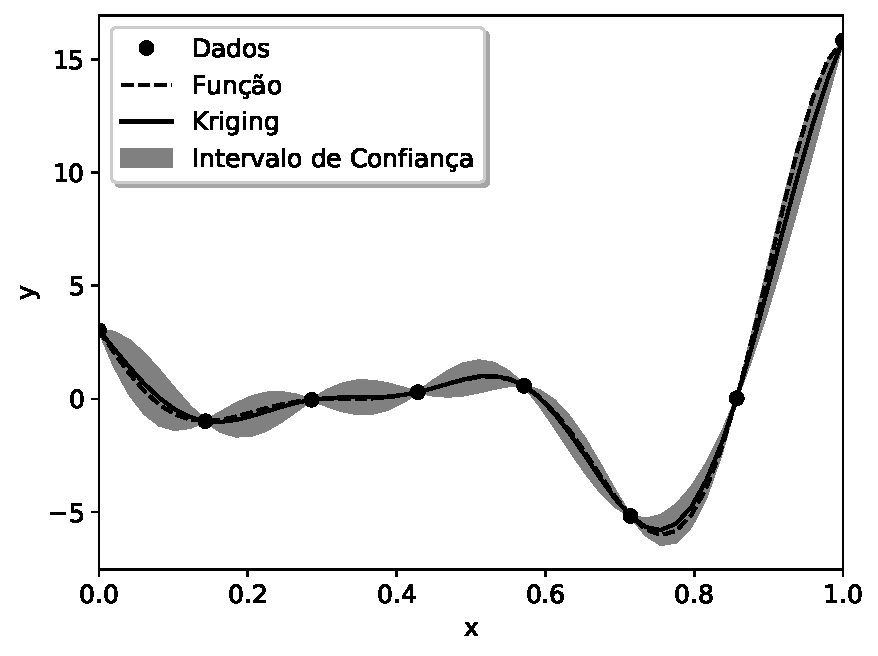
\includegraphics[width=0.7\linewidth]{tatiane/fig_tati/ic/ic1.pdf}} 
	\caption{Intervalo de confiança para o preditor Kriging.} 
	\label{fig:ic}
\end{figure}

\section{Validação de metamodelos}

Ressalta-se que é necessário validar o metamodelo escolhido. Uma forma confiável de fazer isso é utilizando a raiz do erro médio quadrático (\textit{Root Mean Square Error} - RMSE) que é expresso da seguinte forma:
\begin{equation}
RMSE = \sqrt{\frac{\sum_{i=1}^{n_a} ({y_i} - \hat{y_i})^2} {n_a}}
 \label{eq:36}
\end{equation}

\noindent onde $n_a$ representa o tamanho da amostra adicional, $y_i$ é a saída do modelo original e $\hat{y}$ é a saída do metamodelo. 

Destaca-se a existência de outras formas de validar a precisão do metamodelo escolhido como, por exemplo, o coeficiente de determinação $R^2$ dado pela Eq. (\ref{eq:40}) \cite{Erickson2018}.
\begin{equation}
R^{2}= 1-{\frac{\sum_{i=1}^{n_a}({y_i}-\hat{y}_i)^2} {\sum_{i=1}^{n_a}({y_i}-\bar{y}_i)^2}}
\label{eq:40}
\end{equation}